% Created 2022-06-24 Fri 11:36
% Intended LaTeX compiler: pdflatex
\documentclass[11pt]{article}
\usepackage[utf8]{inputenc}
\usepackage[T1]{fontenc}
\usepackage{graphicx}
\usepackage{longtable}
\usepackage{wrapfig}
\usepackage{rotating}
\usepackage[normalem]{ulem}
\usepackage{amsmath}
\usepackage{amssymb}
\usepackage{capt-of}
\usepackage{hyperref}
\usepackage{geometry}
\usepackage{amsmath, amssymb, amsthm, pgfplots, eucal}
\newcommand{\A}{\mathbb{A}}
\renewcommand{\P}{\mathbb{P}}
\renewcommand{\O}{\mathcal{O}}
\renewcommand{\Z}{\mathbb{Z}}
\newcommand{\I}{\mathcal{I}}
\newcommand{\q}{\mathsf{q}}
\newcommand{\Gr}{\textrm{Gr}}
\newcommand{\G}{\mathbb{G}}
\renewcommand{\k}{\mathsf{k}}
\newcommand{\fm}{\mathfrak{m}}
\newcommand{\fp}{\mathfrak{p}}
\renewcommand{\to}{\longrightarrow}
\DeclareMathOperator{\Hom}{\mathsf{Hom}}
\DeclareMathOperator{\sing}{\mathsf{Sing}}
\DeclareMathOperator{\Sym}{\mathsf{Sym}}
\DeclareMathOperator{\V}{\mathcal{V}}
\DeclareMathOperator{\E}{\mathcal{E}}
\DeclareMathOperator{\cubics}{\textrm{cubics}}
\newcommand{\A}{\mathbb A}
\renewcommand{\k}{\mathsf{k}}
\renewcommand{\P}{\mathbb P}
\newcommand{\G}{\mathbb G}
\DeclareMathOperator{\Gr}{Gr}
\renewcommand{\to}{{\longrightarrow}}
\newtheorem{theorem}{Theorem}[section]
\newtheorem{proposition}{Proposition}[section]
\newtheorem{lemma}{Lemma}[section]
\newtheorem{corollary}{Corollary}[section]
\newtheorem{definition}{Definition}[section]
\newtheorem{eg}{Example}[section]
\newtheorem{exercise}{Exercise}[section]
\author{Anand Patel}
\date{\today}
\title{Elements of Classical Algebraic Geometry}
\hypersetup{
 pdfauthor={Anand Patel},
 pdftitle={Elements of Classical Algebraic Geometry},
 pdfkeywords={},
 pdfsubject={},
 pdfcreator={Emacs 26.3 (Org mode 9.5.3)}, 
 pdflang={English}}
\begin{document}

\maketitle

\section{Affine space \(\A^n_{\k}\), algebraic subsets, and the Zariski topology}
\label{sec:org6d41ec3}


Affine varieties are the fundamental building blocks of the objects in classical algebraic geometry, \emph{quasi-projective varieties}.  In essence, an affine variety is the  solution set of a system of polynomial equations with coefficients in some field \(\k\). This solution set is made into a geometric object when we introduce a topology, the \emph{Zariski topology}, on it.  Furthermore, two such solutions sets are allowed to communicate with each other using only a restricted class of functions, called \textbf{\emph{regular maps}}.  Using this, we are then able to codify what it means for two solution sets to be "the same", even though they may arise in totally different contexts.  (Much like in group theory, the notion of homomorphism and isomorphism allows us to witness the same abstract group in various guises.)  An affine variety \(X\) is then defined to be an equivalence class of solution sets under the notion of regular isomorphism, and it turns out that \(X\) is uniquely recoverable from the ring of regular functions on it, called the \emph{coordinate ring}, denoted \(\k[X]\).  The basic philosophy in affine algebraic geometry is then to translate "geometric notions" about \(X\) into ring-theoretic notions about \(\k[X]\), thereby securing geometric intuitions in the rigorous realm of algebra.

The relationship between the originating system of equations and the solution set is tightest when this \emph{ground field} \(\k\) is algebraically closed, and the main theorem(s) describing this relationship is Hilbert's Nullstellensatz in its various incarnations.  

\subsection{Algebraic sets}
\label{sec:orgf9f80b5}

\begin{definition}
\begin{enumerate}
\item \textbf{\emph{Affine space of dimension \(n\) (over \(\k\))}}, denoted \[\A^{n}_{\k}\] is the set of \(n\) -tuples \(p = (p_1, \dots, p_{n})\), \(p_{i} \in \k\).
\item For each \(i\), we denote by \[x_{i}: \A^{n}_{\k} \to \A^{1}_{\k}\] the \(i\)-th coordinate function sending \((p_{1}, \dots, p_{n})\) to \(p_i\).
\item If \(S \subset \k[x_{1} \dots, x_n]\) is a subset of polynomials, we define the \textbf{\emph{vanishing set of \(S\)}} to be
\[\V(S) = \big\{p \in \A^n_{\k} \mid f(p)=0 \, \textrm{for all}\, f \in S \big\}.\]
\item A subset \(U \subset \A^{n}_{\k}\) is a \textbf{\emph{Zariski open set}} if its complement is \(\V(S)\) for some \(S \subset \k[x_1, \dots, x_n]\).
\item Conversely, any subset \(Z \subset \A^n_{\k}\) of the form \(\V(S)\) is called a \textbf{\emph{Zariski closed}} (or, simply \textbf{\emph{closed}}) subset. A Zariski closed subset of affine space also called an \textbf{\emph{algebraic set}}.
\item More generally, if \(Z \subset \A^n_{\k}\) is an algebraic set, then a subset \(U \subset Z\) is  a \textbf{\emph{Zariski open  subset of \(Z\)}} if \(U\) is the intersection of \(Z\) with a Zarski open subset of \(\A^n_{\k}\).
\item A Zariski open subset of an algebraic set is called a \textbf{\emph{quasi-affine set}}.
\end{enumerate}
\end{definition}

The reason for the terminology is: The Zariski open/closed sets satisfy the axioms of a topology.  Whenever we say "open" or "closed" in the context of algebraic sets, we refer to the Zariski topology.  

\begin{eg}
Some algebraic sets are more famous than others (for various reasons), and have names.
\begin{enumerate}
\item The \emph{parabola} \[\V(y-x^{2}) \subset \A^{2}_{\k}.\]
\item The \emph{quadric cone} \[\V(xy-z^2) \subset \A^3_{\k}.\]
\item The \emph{hyperboloid of one sheet} \[\V(xy-z) \subset \A^{3}_{\k}.\]
\item The \emph{nodal cubic} \[\V(y^2 - x^{2}-x^{3}) \subset \A^2_{\k}.\]
\item The \emph{cuspidal cubic} \[\V(y^2-x^3) \subset \A^2_{\k}.\]
\item An / elliptic curve/ \[\V(y^2-x^3+x) \subset \A^2_{\k}.\]
\item The \emph{affine twisted cubic} \[\V(x^2-y,x^3-z) = \V(x^2-y, xy-z) \subset \A^3_{\k}.\]
\item The \emph{Whitney umbrella} \[\V(x^2+zy^2) \subset \A^{3}_{\k}.\]
\end{enumerate}

\begin{center}
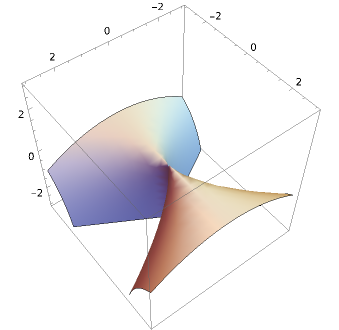
\includegraphics[width=.9\linewidth]{./images/whitney2.png}
\end{center}

\begin{enumerate}
\item A \emph{line and a plane}  \[\V(xz,yz) \subset \A^3_{\k}.\]
\end{enumerate}
\end{eg}


\begin{exercise}
Suppose \(I,J \subset \k[x_1, \dots, x_n]\) are two ideals. Show:
\begin{enumerate}
\item \(\V(I \cdot J) = \V(I) \cup \V(J)\), and
\item \(\V(I+J) = \V(I) \cap \V(J).\)
\item Prove that two distinct ideals \(I\) and \(J\) can satisfy \(\V(I) = \V(J)\), and moreover, there exists an example where neither \(I \subset J\) nor \(J \subset I\).
\item Prove that the Zariski open subsets of \(\A^{n}_{\k}\) satisfy the axioms of a topology. This topology is called the \textbf{\emph{Zariski topology on \(\A^n_{\k}\).}}
\item Prove that the Zariski closed subsets of \(\A^{1}_{\k}\) are the finite sets.
\item If \(S \subset \k[x_1, \dots, x_n]\) is a subset, and if \(\langle S \rangle\) denotes the ideal generated by \(S\), then prove that \(\V(S) = \V(\langle S \rangle)\).
\item Prove that every finite subset of \(\A^{n}_{\k}\) is closed, but that the converse is not true for all \(n \geq 2\).
\end{enumerate}
\end{exercise}

In light of this exercise, in order to create an algebraic set, we need only consider \(\V(I)\)'s for \emph{ideals} \(I \subset \k[x_1, \dots,
x_n]\).

And so, the operation \(\V\) therefore provides a surjective function: \[\V(-): \big\{\,\textrm{ideals} \,\, I \subset \k[x_1, \dots, x_n] \big\} \to \big\{\,\textrm{algebraic sets} \,\, X \subset \A^{n}_{\k} \big\}.\]

We can also go backwards, from sets to ideals:

\begin{definition}
Let \(Z \subset \A^n_{\k}\) be any subset.  We define the \textbf{\emph{ideal of \(Z\)}} to be \[I(Z) = \big\{ f \in \k[x_1,\dots,x_n] \mid f(z)=0\,\, \textrm{for all}\,\,z \in Z \big\}.\]
\end{definition}

\begin{eg}
Let \(p = (p_1, \dots, p_n) \in \A^n_{\k}\) be any point. Then \(I(\{p\}) = (x_1-p_1, \dots, x_n-p_n)\). Notice that \(I(\{p\}) \subset \k[x_1,\dots, x_n]\) is a \emph{maximal ideal}.  So, we typically use the symbol \(\fm_p\) for this ideal.
\end{eg}


\begin{exercise}
\begin{enumerate}
\item Prove: For any subset \(Z \subset \A^{n}_{\k}\), we have \(Z \subset \V(I(Z))\).
\item Prove:  \(Z \subset \A^n_{\k}\) is Zariski-closed if and only if \(Z = \V(I(Z))\).
\item In fact, prove: For any \(Z \subset \A^n_{\k}\), \(\V(I(Z))\) is the closure of \(Z\) under the Zariski topology on \(\A^n_{\k}\).
\end{enumerate}
\end{exercise}

\subsection{Regular functions}
\label{sec:orged41503}

Next, we must set the rules for how algebraic sets and quasi-affine sets are allowed to communicate with each other. In short, we allow ourselves, to the extent that it is possible, to use functions which are describable using polynomials and their ratios.  These functions are called regular functions.

\begin{definition}
Let \(U \subset Z\) be an open subset of an algebraic set.
\begin{enumerate}
\item A function \(f: U \to \A^1_{\k}\) is \textbf{\emph{regular}} if: for every \(x \in U\), the function \(f\) agrees with a ratio of polynomials \(p/q\) (with \(q(x) \neq 0\)) on some open subset \(V \subset U\) containing \(x\). The ring of regular functions on \(U\) is denoted \(\k[U]\).
\item A map \(\varphi = (f_1, \dots, f_m): U \to \A^m_{\k}\) is \textbf{\emph{regular}} if each coordinate function \(f_i\) is in \(\k[U]\).
\item If \(V \subset W\) is another quasi-affine set, with \(W\) an algebraic subset of \(\A^m_{\k}\), then a \textbf{\emph{regular mapping}} \(\varphi: U \to V\) is a regular map \(\varphi: U \to \A^m_{\k}\) whose image lies in \(V\).
\end{enumerate}
\end{definition}

\begin{proposition}
If \(U\) and \(V\) are quasi-affine sets, and if \(\varphi: U \to V\) is a regular mapping, then \(\varphi\) is continuous for the Zariski topologies on \(U\) and \(V\), i.e. the preimage of any closed set is closed.
\end{proposition}

\begin{exercise}
Let \(\varphi: U \to V\) be a regular mapping between quasi-affine sets.  Prove:
\begin{enumerate}
\item If \(g \in \k[V]\)  then \(g \circ \varphi \in \k[U]\).
\item The formula \(g \mapsto g \circ \varphi\) defines a \(\k\)-algebra homomorphism \(\k[V] \to \k[U]\).
\item If \(U\) and \(V\) are affine sets, then, conversely, any homomorphism \(\k[V] \to \k[U]\) comes from a regular mapping \(g: U \to V\).
\end{enumerate}
\end{exercise}


\begin{theorem}
Let \(Z \subset \A^n_{\k}\) be an algebraic set. Then every regular function on \(Z\) is the restriction of a polynomial.  Thus, the ring of regular functions on \(Z\) is isomorphic to \(\k[x_1, \dots, x_n]/\I(Z)\). 
\end{theorem}

\begin{exercise}
Let \(Z \subset \A^n_{\k}\) be an algebraic subset, and let \(f \in \k[x_0, \dots, x_n]\) be any polynomial.  If \(\varphi: Z_f \to \A^1_{\k}\) is a regular function then there exists a polynomial \(a\) such that \(p = a/f^{m}\) for some \(m \geq 0\). 
\end{exercise}

\subsection{Hilbert's Nullstellensatz}
\label{sec:orgdce084b}

Our first fundamental  theorem, which appears in several different forms in several different levels of generality, explains the relationship between the operations \(\V(-)\) and \(I(-)\).  The exact message of Hilbert's Nullstellensatz can be confusing for newcomers, so I'll try to summarize the situation here:

\begin{enumerate}
\item When \(\k\) is algebraically closed, the Nullstellensatz tells us that the only way for \(\V(I)\) to be empty is if \(I = (1)\), the unit ideal. In other words, any system of polynomial equations which is not equivalent to \(1=0\) \textbf{\emph{must have}} solutions in \(\A^n_{\k}\).
\item When \(\k\) is algebraically closed, the Nullstellensatz provides the precise list of \emph{maximal ideals in} \(\k[x_1, \dots, x_n]\).
\end{enumerate}

\begin{theorem}
Let \(\k\) be an arbitrary field.

\begin{enumerate}
\item If \(L\) is a finitely generated \(\k\)-algebra which is also a field, then \(L\) is a finite field extension of \(\k\).

\item A polynomial system of equations \(\big\{f_1=0, f_2=0, \dots, f_m =0 \big\}\) with \(f_i \in \k[x_1, \dots, x_n]\) has a solution in \textbf{\emph{some}} \(\k\)-algebra if and only if it has a solution \((\alpha_1, \dots, \alpha_n)\) where each \(\alpha_i\) is algebraic over \(\k\).

\item If \(\k\) is algebraically closed, then every maximal ideal of \(\,\,\k[x_1, \dots, x_n]\) is of the form \((x_1-p_1, \dots, x_n-p_n)\) for some \(p_i \in \k\).

\item If \(\k\) is algebraically closed, and if \(I \subset \k[x_1, \dots, x_n]\) satisfies \(\V(I) = \emptyset\), then \(I = (1)\), the unit ideal.
\item If \(\k\) is algebraically closed, and if \(\fp \subset \k[x_1, \dots, x_n]\) is a prime ideal, then \(I(\V(\fp)) = \fp\).
\end{enumerate}
\end{theorem}


\begin{exercise}
Let \(\k[x]\) denote the polynomial ring in one variable, and suppose \(f_1, \dots, f_m \in \k[x]\) are finitely many polynomials.  Prove that the ring \(\k[x, \frac{1}{f_1}, \dots, \frac{1}{f_m}]\) is never a field. 
\end{exercise}


\subsubsection{Some  algebra: finite/integral extensions of rings}
\label{sec:org5c37bcf}

\begin{definition}
\begin{enumerate}
\item An extension \(A \subset B\) of rings is \textbf{\emph{an integral extension}} if every element of \(B\) satisfies a monic polynomial with coefficients in \(A\).

\item An extension of rings \(A \subset B\) is \textbf{\emph{finite}} if \(B\) is finitely generated as an \(A\)-module.
\end{enumerate}
\end{definition}

\section{Projective space \(\P^n_{\k}\) and projective varieties}
\label{sec:orgf228950}
For a multitude of reasons, it is useful to want to \emph{compactify} affine space.  Take, for instance, the concept of the \emph{slope of a line} from high school algebra.  Slopes were numbers, typically labelled \(m\).  Except, hold on, what about those pesky "vertical" lines?  It is clear that, geometrically, vertical lines are no more special than any other kind of line.  So we should extend the concept of slope \(m\) to include an "infinity" slope \(m =\infty\). By adding \(\infty\) to the \(\A^1\) of slopes, we arrive at the \emph{projective line} \(\P^1\).

Another way that projective space arises is in the following context:  We have a vector space \(V\), but we only really care  about elements of \(V\) \emph{up to scaling}.  For instance, if we only care about the \emph{location of the roots} of a quadratic polynomial \(ax^2+bx+c\), then for our purposes there is no difference between polynomials \(ax^2+bx+c\) and \(\lambda a x^2 + \lambda b x + \lambda c =0\), where \(\lambda\) a nonzero number.
\subsection{Projective varieties}
\label{sec:org6ea3458}
For simplicity, we work throughout over an algebraically closed field \(\k\).

\begin{definition}
\begin{enumerate}
\item The \(n\)-dimensional projective space, denoted \(\P^n_{\k}\), is the set of equivalence classes of points of \(\left(\A^{n+1}_{\k}\right)^{\times}\) under the action of \(\k^{\times}\) by scaling.
\item A point \(p \in  \P^n_{\k}\) is denoted by a tuple \([p_0 : p_1 : \ldots : p_n]\), and two tuples \([p_0 : p_1 : \ldots : p_n]\) and \([q_0 : q_1 : \dots : q_n]\) represent the same point in \(\P^n_{\k}\) if and only if there exists \(\lambda \in \k^{\times}\) such that \(p_i = \lambda q_i\) for all \(i = 0,\ldots, n\).
\item The assignment \((p_0, \dots, p_n) \mapsto [p_0 : \dots : p_n]\) defines the \textbf{\emph{quotient mapping}} \[\q : \left( \A^{n+1}_{\k}\right)^{\times} \to \P^n_{\k}.\]
\item The \textbf{\emph{Zariski topology on \(\P^n_{\k}\)}} is defined as follows: A subset \(U \subset \P^n_{\k}\) is open (resp. closed) if and only if \(\q^{-1}(U)\) is Zariski-open (resp. closed) in  \(\left( \A^{n+1}_{\k}\right)^{\times}\).
\item For each \(i=0, \ldots, n\), we define the \textbf{\emph{\(i\)-th standard affine open chart of \(\P^n_{\k}\)}} to be the open set \[U_{i} = \big\{ [p_{0}: \ldots : p_n] \mid p_i \neq 0 \big\}.\]
\end{enumerate}
\end{definition}

\begin{exercise}
\begin{enumerate}
\item For each \(i=0,\ldots, n\), let \(\gamma_i: \A^{n}_{\k} \to U_i\) denote the bijective function that sends \((a_0, \ldots, a_{i-1}, a_{i+1}, \ldots a_n)\) to the point \([a_0: \ldots: a_{i-1} : 1 : a_{i+1} : \ldots : a_n]\).  Prove that \(\gamma_i\) is a \emph{homeomorphism} of topological spaces, meaning: \(Y \subset \A^n_{\k}\) is Zariski-open if and only if \(\gamma_i(Y) \subset U_i\) is Zariski-open.
\item One could define another topology on \(\P^n_{\k}\) in the following way: A set \(Y \subset \P^n_{\k}\) is closed if and only if \(Y_{i} := Y \cap U_i\) is closed in \(U_i\) for all \(i\), where we think of \(U_i\) as an affine space under the indentifications \(\gamma_i\) in the previous exercise.  Prove that this topology is the same as the Zariski topology defined in the definition above.
\end{enumerate}
\end{exercise}


\begin{theorem}
Every closed subset of  \(\P^{n}_{\k}\) is obtained as the vanishing set of a graded ideal in \(\k[X_0, \dots, X_n]\). 
\end{theorem}
\subsection{Projective morphisms}
\label{sec:orga3c073f}
\begin{theorem}
The main theorem of elimination theory.
\end{theorem}
\subsection{Morphisms between projective spaces}
\label{sec:org5a22a68}

\begin{definition}
Let \(X, Y\) be two varieties, with \(X\) irreducible. A \textbf{\emph{rational map}} from \(X\) to \(Y\), is an equivalence class of pairs \((\varphi, U)\) where:
\begin{enumerate}
\item \(U \subset X\) is a non-empty open set, and \(\varphi: U \to Y\) is a regular map, and
\item Two pairs \((\varphi, U)\) and \((\xi, V)\) are equivalent if there exists an open subset \(W \subset U \cap V\) where \(\varphi|_{W} = \xi|_{W}\).
\end{enumerate}
\end{definition}

\begin{proposition}
Let \(\varphi: X \dashrightarrow Y\) be a rational map.  Then there exists a maximal domain of definition, \(U_{\textrm{max}} \subset X\) for \(\varphi\), i.e. if \((\xi,U)\) represents \(\varphi\) then \(U \subset U_{\textrm{max}}\). 
\end{proposition}

(Proof: For all representatives \((\xi_{\alpha}, U_{\alpha})\) representing \(\varphi\), define \(U_{\textrm{max}}\) to be the union of all \(U_\alpha\). Suppose \((\xi_{\alpha}, U_{\alpha})\) and \((\xi_{\beta}, U_{\beta})\) both represent \(\varphi\). Then \(U_{\alpha} \cap U_{\beta}\) is an irreducible quasi-projective variety.  The two regular maps \(\xi_{\alpha}|_{U_{\alpha} \cap U_{\beta}}\) and \(\xi_{\beta}|_{U_{\alpha} \cap U_{\beta}}\) agree on an open set, and therefore agree everywhere.  Thus the \(\xi_{\alpha}\)'s glue together to produce a regular map on \(U_{\textrm{max}}\), which is what we needed.)


\begin{theorem}
Every regular mapping \(\varphi: \P^n_{\k} \to \P^m_{\k}\) is of the form \([x_0, \dots, x_n] \mapsto [F_0: \ldots : F_m]\) for some homogeneous forms \(F_{i}\) of the same degree, not all sharing a common zero.
\end{theorem}

\begin{theorem}
Every regular automorphism of \(\P^n_{\k}\) is a linear change of variables.
\end{theorem}

\section{Tangent spaces}
\label{sec:org725e215}
To each point \(x\) on a variety \(X\) we attach a \(k\)-vector space \(T_{X,x}\), called the \textbf{\emph{Zariski tangent space}}.   This vector space unlocks the concept of \textbf{\emph{smoothness}} of \(X\) at \(x\), which is the  algebro-geometric formulation of the intuition that \(X\) appears ``locally linear" around \(x\). 


\begin{definition}
Let \(x \in X\) be a point on a variety.  The \textbf{\emph{Zariski tangent space of \(X\) at \(x\)}}, denoted \(T_{X,x}\), is the \(\k\)-vector space \[\left( {\fm_{x}}/{\fm_{x}^2} \right)^{\vee}.\]
\end{definition}

The ring \(\k[\varepsilon]/(\varepsilon^2)\) provides a sometimes-useful alternate interpretation of the Zariski tangent space.  This is encoded in the following critical exercise. 

\begin{exercise}
Let \(x \in X\) be a point on a variety. Then there is a canonical identification between \(T_{X,x}\) and the set of \$\k\$-algebra homomorphisms \(\phi : \O_{X,x} \to \k[\varepsilon]/(\varepsilon^2)\) which send \(\fm_{x}\) into the ideal \((\varepsilon)\).
\end{exercise}

\subsection{Singular points and smooth points}
\label{sec:org0b0b5a2}

\subsection{The nature of the local ring at a smooth point}
\label{sec:org3f941b1}

\subsection{Bertini's theorem(s)}
\label{sec:orgd5ab332}

\begin{theorem}
Let \(f: X \to \P^n_{\k}\) be a map from a smooth, quasi-projective variety \(X\) to a projective space, and suppose \(\k\) is a \textbf{\emph{perfect}}, algebraically closed field.  If \(H \subset \P^n_{\k}\) is a Zariski-general hyperplane, then \(f^{-1}(H) \subset X\) is a smooth divisor.
\end{theorem}




\section{Constancy of number}
\label{sec:org2cba497}

\begin{theorem}
Let \(f: X \to Y\) be a finite map, with \(X\) and \(Y\) smooth, irreducible affine varieties over a characteristic zero field. Then the length of every fiber is equal to the degree of \(f\). (Degree of extension fields.)
\end{theorem}

\section{Hypersurfaces}
\label{sec:orgb2ed85c}

Let \(X = \V(F) \subset \P^n_{\k}\) be a hypersurface, defined by a degree \(d\) homogeneous form \(F(x_0, \dots, x_n)\).   Let \(p = (p_0, \ldots, p_n) \in \left( \A^{n+1} \right)^{\times}\) be a point such that \(F(p) = 0\), and let \(\hat{X} \subset  \A^{n+1}\) denote the affine cone over \(X\).  Then \(X\) is singular at \([p]\) if and only if \(\hat{X}\) is singular at \(p\). 
\section{Basics on vector bundles}
\label{sec:org2fb6c44}
\subsection{The definition of a vector bundle}
\label{sec:org86d9171}
The concept of a \textbf{\emph{vector bundle}} is ubiquitous in mathematics, and captures the idea of a "family of vector spaces parametrized by a base space."  In algebraic geometry, the definition is as follows:
\begin{definition}
Let \(X\) be a variety.  A \textbf{\emph{rank \(r\) vector bundle over \(X\)}} is a variety \(\E\) together with a regular map \(\pi: \E \to X\) such that:
\begin{itemize}
\item There is an open covering \(\{U_{\alpha}\}\) of \(X\)  and isomorphisms \(\phi_{\alpha}: \pi^{-1}(U_{\alpha}) \to U_{\alpha}\times \A^r_{\k}\) TODO
\end{itemize}
\end{definition}
\subsection{Line bundles}
\label{sec:org256547f}
\subsubsection{Line bundles on \(\A^n_{\k}\).}
\label{sec:orgc9c3e10}
Curiously, for affine varieties, the capacity for carrying interesting lines bundles is related to unique factorization.
\begin{theorem}
Every line bundle on \(\A^{n}_{\k}\) is isomorphic to the trivial line bundle.
\end{theorem}
\subsubsection{Line bundles on \(\P^n_{\k}\).}
\label{sec:org42f55a9}

\begin{definition}
Fix an integer \(d \in \Z\). The line bundle \(\O(d)\) on \(\P^{n}_{\k}\) is\ldots{}TODO 
\end{definition}

\begin{theorem}
Every line bundle on \(\P^n_{\k}\) is isomorphic to one of the line bundles \(\O(d)\).
\end{theorem}
\section{The basic geometry of Grassmannians}
\label{sec:org4e90a75}
\section{Algebraic Geometry in Linear Algebra}
\label{sec:orged4e243}
\subsection{Rank-dropping varieties}
\label{sec:orgc375af0}

Suppose \(V\) and \(W\) are \(\k\)-vector spaces of dimensions \(n\), and \(m\) respectively.  In this document we will establish fundamental facts about the geometry of a particularly ubiquitous stratification of the vector space of linear homomorphisms \[\Hom(V,W)\]


\begin{definition}
For each integer \(r \leq m\), we define the subset $$\mathsf{R}_{r} \subset \Hom(V,W)$$ as the collection of homomorphisms \(\varphi: V \to W\) having rank \(\leq r\).  Furthermore, let $$\mathring{\mathsf{R}}_{r} = \mathsf{R}_{r}\setminus \mathsf{R}_{r-1}$$ be the set of homomorphisms of rank \(r\).
\end{definition}


On the extremes, \(\mathsf{R}_m = \Hom(V,W)\) and \(\mathsf{R}_{0} = \{0\}\).  After choosing bases of \(V\) and \(W\), every element of \(\Hom(V,W)\) is represented by a \(m \times n\) matrix. Let us write the \textbf{\emph{universal \(m \times n\) matrix}} as 
\[A = \big\{ x_{ij} \big\} \,\,\,  1 \leq i \leq m, 1 \leq j \leq n.\]
Linear algebra says: 

For each \(r\), the subset \(\mathsf{R}_{r}\) is the common vanishing locus of all determinants of \((r+1) \times (r+1)\) minors of the universal matrix \(A\).

Thus, \(\mathsf{R}_{r}\) is a sub-variety of \(\Hom(V,W)\).  (In fact, it comes with a "usual" scheme structure given by the ideal in \(\k\left[\{X_{i,j}\}\right]\) generated by \((r+1) \times (r+1)\)-minors of \(A\).) 



\begin{exercise}
In light of the canonical identification between \(\Hom(V,W)\) and \(\Hom(W^{\vee},V^{\vee})\), why is it enough to study the situation where \(n \leq m\)?
\end{exercise}


\begin{exercise}
Let \(I_{r} \subset \k[\{ x_{ij}\}]\) denote the ideal generated by the determinants of the \((r+1) \times (r+1)\) minors of \(A\).  Prove that \(I_{r-1}\) is generated by all partial derivatives of all elements in the ideal \(I_{r}\).
\end{exercise}


In the language of schemes, this translates to: \emph{\(\mathsf{R_{r-1}}\) is
the singular scheme of \(\mathsf{R_{r}}\).}






\begin{exercise}
Examine the geometry of the subvarieties \(\mathsf{R}_{r}\) when \(m=n=2\).
\end{exercise}

\subsubsection{The relevant incidence variety}
\label{sec:orgcbe6583}
For each \(1 \leq r \leq m\) we define the subset 
\[\widetilde{\mathsf{R}}_{r} \subset \Hom(V,W) \times \Gr(n-r,V)\] as the set of pairs \((\varphi, \Lambda)\)  satisfying  \[ \Lambda \subset \ker \varphi.\]


Let \(\pi_{1}: \widetilde{\mathsf{R}}_{r} \to \Hom(V,W)\) denote the projection onto the first factor, \(\pi_{1}(\varphi, \Lambda) := \varphi\).  Then \(\pi_{1}\) is a projective morphism, and \(\pi_{1}(\widetilde{\mathsf{R}}_{r}) = \mathsf{R}_{r}\).


\begin{exercise}
\begin{enumerate}
\item Prove, using standard affine charts on the \(\Gr(n-r,V)\), that \(\widetilde{\mathsf{R}}_{r}\) is a closed subvariety of \(\Hom(V,W) \times \Gr(n-r,V).\)  For a follow-up exercise, show it is irreducible.
\item Prove that \(\pi_{1}: \widetilde{\mathsf{R}}_{r} \to \mathsf{R}_{r}\) is an isomorphism over \(\mathring{\mathsf{R}}_{r}\).
\item (\(\varepsilon\)asy  with \(\varepsilon\)-skills.) Let \((\varphi, \Lambda)\) denote an arbitrary point of \(\widetilde{\mathsf{R}}_{r}\). Then the tangent space of \(\widetilde{\mathsf{R}}_{r}\) at \((\varphi, \Lambda)\) is the subspace of   \(Hom(V,W) \oplus Hom(\Lambda, V/\Lambda)\) consisting of pairs \((\psi,\alpha)\) such that \[\overline{\varphi} \circ \alpha + \psi|_{\Lambda} = 0\] as elements of \(Hom(\Lambda, W)\).  Here, \(\overline{\varphi}: V /\Lambda \to W\) is the map induced by \(\varphi\).
\end{enumerate}
\end{exercise}

The conclusion from all exercises above is: 

\begin{theorem}
Theorem on the Geometry of Rank-Dropping: 
\begin{enumerate}
\item The variety \(\widetilde{\mathsf{R}}_{r}\) is smooth and irreducible.
\item The map \(\pi_{1}: \widetilde{\mathsf{R}}_{r} \to \mathsf{R}_{r}\) is an isomorphism precisely over  \(\mathring{\mathsf{R}}_{r}\).  Hence, \(\mathsf{R}_{r}\) is irreducible, and has codimension \((n-r)(m-r)\) in \(\Hom(V,W)\).
\item \(\sing(\mathsf{R}_{r}) = \mathsf{R}_{r-1}\).
\end{enumerate}
\end{theorem}

\subsection{Symmetric linear algebra and the geometry of quadric hypersurfaces}
\label{sec:org19a8581}

Let \(V\) be an \((n+1)\)-dimensional vector space \textbf{\emph{over a ground field \(\k\) of characteristic not \(2\).}}

Let \(Q \in \Sym^{2}V^{\vee}\) be a quadratic form on \(V\). Choose a basis \((v_{i})_{i=0, \ldots, n}\) of \(V\), and the corresponding dual basis \((X_{i})\) of \(V^{\vee}\).  Then, the quadratic form \(Q\) is a homogeneous quadratic polynomial \(Q(X_0, \ldots, X_n)\), and defines a corresponding quadric hypersurface $$\mathsf{Q} \subset \P V$$ defined as the vanishing (scheme) of \(Q\).


\begin{definition}
The \textbf{\emph{rank of \(Q\)}} (or \textbf{\emph{the rank of \(\mathsf{Q}\)}}) is defined to be the rank of the symmetric matrix \(S(Q)\).
\end{definition}


\begin{exercise}
\begin{enumerate}
\item The singular locus (scheme) of \(\mathsf{Q}\) is a linear space, and is the projectivization of the kernel of the \((n+1)\times(n+1)\)-symmetric matrix \(S(Q)\).

\item \(\mathsf{Q}\) is smooth if and only if it has full rank (\(= n+1\)). In general, \(\sing(\mathsf{Q}) \subset \P V\) is a linear space with codimension equal to the rank of \(\mathsf{Q}\).

\item Using the fact that over an algebraically closed field all  symmetric matrices are diagonalizable, show that over such a field (characteristic not = \(2\)), every quadric is projectively equivalent to exactly one of the \((n+1)\) quadrics from the list:
\item Suppose \(\mathsf{Q} \subset \P V\) is a quadric hypersurface with \(\dim \sing(\mathsf{Q}) = s \geq 0\).  Then there is a choice of homogeneous coordinates \((X_0, \dots, X_{n})\) of \(V\) in terms of which \(\mathsf{Q}\) has defining equation of the form $$Q(X_0, \ldots, X_n) = \sum_{i = 0}^{n-s-1}X_{i}L_{i}$$ where \(L_{i}\) are linear forms in the variables \(X_0, \ldots, X_{n-s-1}\), and furthermore such that the common vanishing space of the \(L_{i}\) is the plane \(X_0 = \dots = X_{n-s-1}=0\).
\end{enumerate}
\[X_{0}^{2},\,\,\, X_{0}^2+X_{1}^2,\,\, \ldots\,\,\,, X_{0}^{2} + X_{1}^2 + \cdots +X_{n}^{2}.\]
\end{exercise}
\section{The geometry of smooth cubic surfaces}
\label{sec:org4b4bdbb}
The geometry of smooth cubic surfaces is extremely rich and interesting, and constitutes one of the earliest chapters  in classical algebraic geometry.  The first fundamental theorem, due to Cayley and Salmon, is: 

\begin{theorem}
A cubic surface \(X \subset \P^3\) contains exactly \(27\) lines if and only if it is smooth. 
\end{theorem}


\begin{definition}
Define the \textbf{\emph{cubic-line}} incidence correspondence to be the subset \[\Sigma \subset \P^{19}_{\cubics} \times \G(1,3)\] consisting of those pairs \((X,\ell)\) where \(X\) is a cubic surface and \(\ell\) is a line contained in \(X\).
\end{definition}

\begin{exercise}
In this exercise, we assume the ground field \(\k\) is algebraically closed (arbitrary characteristic). 
\begin{enumerate}
\item Prove that \(\Sigma\) is a smooth, \(19\)-dimensional variety by considering the structure of the second projection \(\pi_2:\Sigma \to \G(1,3)\).
\item Let \(L\) denote the line \(x_0 = x_1 = 0\).  Show that any cubic \(X\) containing \(L\) is of the form \(\V(F)\) where \(F = x_0 \cdot Q_0 + x_1 \cdot Q_1\), where \(Q_i(x_0,x_1,x_2,x_3)\) are quadratic forms, and that \(X\) is singular at a point \(p \in L\) if and only if \(Q_0(p) = Q_1 (p) = 0\).
\item Prove that a line \(L\) on a cubic surface \(X\) admits a non-trivial first order deformation \textbf{\emph{within \(X\)}} if and only if there is a point \(p \in L\) where \(X\) is singular.
\item Prove that if \(p \in X\) is a singular point on a cubic surface then there must be a line \(L \subset X\) containing \(p\).
\item Conclude that the first projection \[\pi_{1}: \Sigma \to \P_{\cubics}^{19}\] is unramified at every point of \(\pi_{1}^{-1}([X])\) if and only if \(X\) is a smooth cubic surface.
\item From the \textbf{\emph{Theorem on Conservation of Number}}, conclude that \emph{every smooth cubic surface contains the same number of lines as every other smooth cubic, and every singular cubic either contains strictly fewer lines, or infinitely many.}
\item Finally, by considering the particularly beautiful  cubic surface \(\V(x_{0}^2x_{1} + x_{1}^2x_{2} + x_{2}^{2}x_{3}+ x_{3}^{2}x_{0})\) conclude the theorem of Cayley and Salmon: \emph{A cubic surface contains exactly \(27\) lines if and only if it is smooth.} (This cubic, the Clebsch cubic, has lines defined over \(\Z[\zeta_{5}]\), so it might be challenging to find the lines. It is also singular over \(\mathbb{F}_{5}\), which is consistent with the fact that \(\Z[\zeta_{5}]\) is ramified only over \(5\).)
\end{enumerate}
\end{exercise}
\end{document}
